\documentclass[../../main.tex]{subfiles}

\begin{document}

	\subsection{Reliability}

	CLup's queueing system is critical in order to keep track of the accesses, thus its infrastructure 
	should be characterized by the highest MTTF and lowest MTTR possible.

	A larger MTTR is acceptable for the other services, however it's mandatory to ensure the lack of 
	data losses during downtime.

	\subsection{Availability}

	All services must be up and running 24/7, both supermarkets and users need to be notified in case of 
	any communication issues with CLup servers.

	Stores should be able to communicate with CLup's servers during all their opening time span.

	As shown in the following histogram, it is expected an high utilisation of all services during the day, 
	and a low usage during night hours.

	\begin{figure}[h!]
	    \centering
	    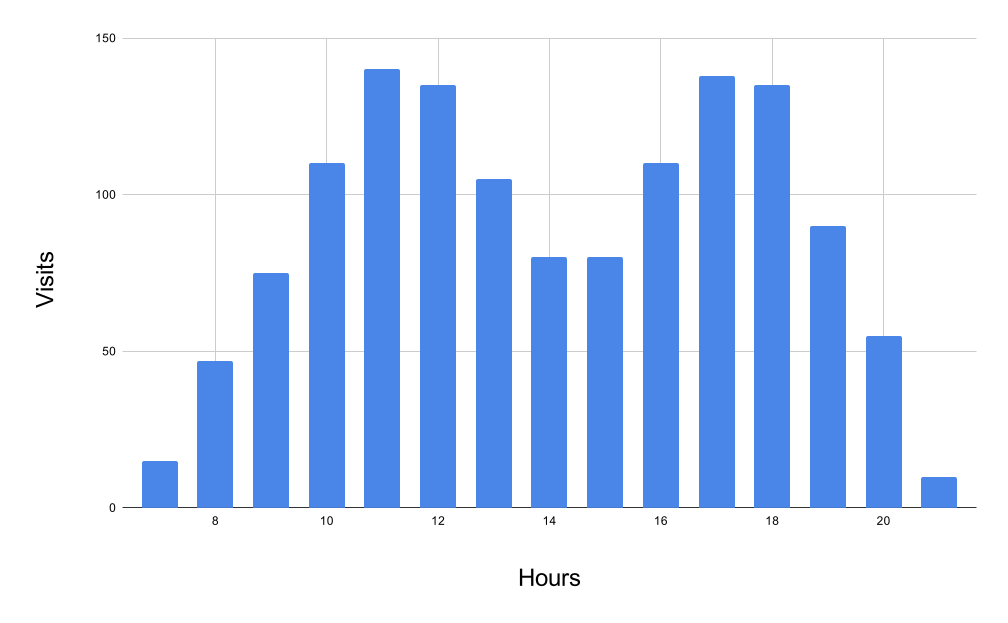
\includegraphics[width=0.8\textwidth]{affluence-chart.png}
	    \caption{Average daily visits in the biggest supermarket in Milan. \\Credits: Google.}
  	\end{figure}

	\subsection{Security}

	All data inbound to CLup services must be treated as stated by security regulations. 

	Store personnel (i.e., store managers and store assistants) will authenticate to the system using Single Sign On (SSO) integrations with the stores identity systems, using either OAuth or SAML. This will allow the system to delegate the user management to external identity systems, with the benefits of:
	- not having to deal with sensitive information (e.g., passwords)
	- inheriting the change of permissions of the users (e.g., a promotion from store assistant to store manager)
	- providing the users with a unified and smooth log in experience (since they will use the same credentials they use to access all other stores' systems)

	Additionally, in order to guarantee the protection of the customer's data in between servers and the 
	user's device, all Internet traffic must be encrypted with a modern version of TLS, and sent via HTTPS protocol.


	\subsection{Maintainability}

	The back-end system must be designed in order for sustaining maintainance operations without having to 
	shut down services, guaranteeing no down-time during these operations. For this reason, a dedicated staging environment must be put in place and used to test every new release of the software. The staging environment must be as similar as possible to the production environment, the only difference being the data that it works on: properly anonymized production data.

	All devices inside the supermarkets, like ticket scanners and printers, must support OTA firmware update. These devices can only be updated if necessary, and only when the store is closed.

	Customer's software on smartphones can be updated at any time, through the appropriate app stores.

	\subsection{Portability}

	CLup smartphone application must be available for Android and iOS operating systems. As per compatibility, the Android app must be supported by at least Android KitKat 4.4, while the iOS app must be compatible with at least iOS 12.4.

	All functions available for customers must also be present on Web platform, in order to be able to access 
	CLup's services by Internet browsers, both from PC and smartphones.

	The software for store managers and employees must be hosted on Web platform, with support for both PC and smartphone layouts.

	
\end{document}
